\newcommand{\figuraPotencialLennardJones}{%
\begin{figure}[htbp]
    \centering
    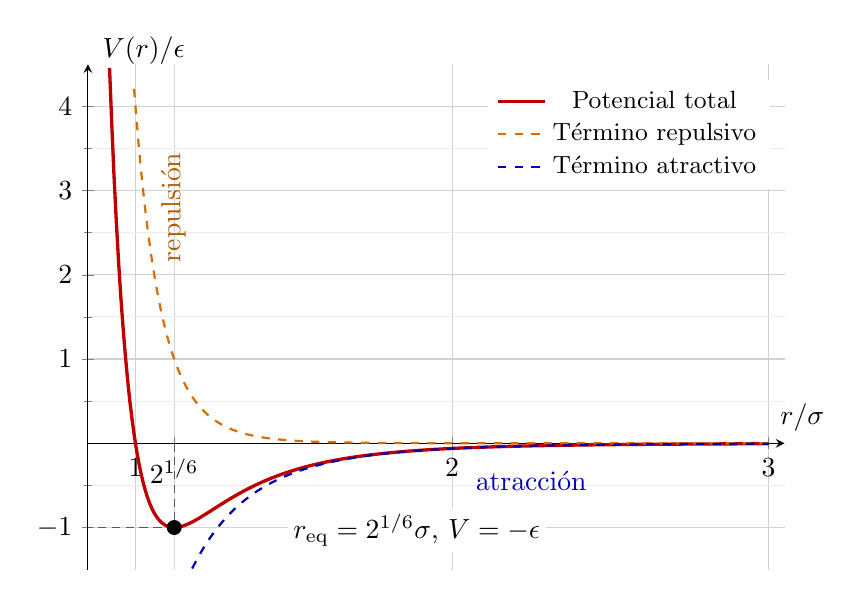
\begin{tikzpicture}
        \begin{axis}[
            width=0.86\textwidth,
            height=8cm,
            axis lines=middle,
            xmin=0.85,
            xmax=3.05,
            ymin=-1.5,
            ymax=4.5,
            xlabel={$r/\sigma$},
            ylabel={$V(r)/\epsilon$},
            xlabel style={at={(axis description cs:0.98,0.30)},anchor=west},
            ylabel style={at={(axis description cs:0.08,0.98)},anchor=south},
            xtick={1,1.12246,2,3},
            xticklabels={$1$,$2^{1/6}$,$2$,$3$},
            ytick={-1,0,1,2,3,4},
            grid=both,
            minor tick num=1,
            major grid style={gray!35},
            minor grid style={gray!15},
            samples=300,
            domain=0.89:3,
            restrict y to domain=-1.5:4.5,
            legend style={
                at={(0.98,0.97)},
                anchor=north east,
                draw=none,
                fill=white,
                font=\small
            }
        ]
            \addplot[very thick,red!75!black]
                {4*(x^(-12)-x^(-6))};
            \addlegendentry{Potencial total}

            \addplot[thick,dashed,orange!85!black]
                {4*x^(-12)};
            \addlegendentry{Término repulsivo}

            \addplot[thick,dashed,blue!70!black]
                {-4*x^(-6)};
            \addlegendentry{Término atractivo}

            \addplot[only marks,mark=*,mark size=2.5pt,black]
                coordinates {(1.12246,-1)};
            \draw[densely dashed,black!65]
                (axis cs:1.12246,0)--(axis cs:1.12246,-1)
                --(axis cs:0.85,-1);
            \node[anchor=south west,fill=white,inner sep=2pt]
                at (axis cs:1.48,-1.30)
                {$r_{\mathrm{eq}}=2^{1/6}\sigma$, $V=-\epsilon$};

            \node[rotate=90,text=orange!70!black]
                at (axis cs:1.12,2.8) {repulsión};
            \node[text=blue!70!black]
                at (axis cs:2.25,-0.45) {atracción};
        \end{axis}
    \end{tikzpicture}
    \caption{Potencial de Lennard--Jones en variables adimensionales. A
    distancias cortas domina el término repulsivo $r^{-12}$; a distancias
    mayores domina el término atractivo $-r^{-6}$. El mínimo corresponde a la
    separación molecular de equilibrio.}
    \label{fig:potencial-lennard-jones}
\end{figure}%
}
